\documentclass[8pt,landscape]{article}
\usepackage{multicol}
\usepackage{calc}
\usepackage{ifthen}
\usepackage[landscape]{geometry}
\usepackage{amsmath,amsthm,amsfonts,amssymb}
\usepackage{color,graphicx,overpic}
\usepackage{hyperref}
\usepackage{graphicx}
\usepackage{amsmath}
\usepackage{tabularx}
\graphicspath{ {sheet_images/} }

\renewcommand\tabularxcolumn[1]{m{#1}}

%Originally Modified by Daniel Kenner for Calc 3 Cheat Sheet
%Template Originally found @ http://tex.stackexchange.com/questions/8827/preparing-cheat-sheets
%Conic images originally found on google images when looking for named shapes

\pdfinfo{
  /Title (Calculus 3 Cheat Sheet.pdf)
  /Creator (TeX)
  /Producer (pdfTeX 1.40.0)
  /Author (Daniel Kenner)
  /Subject (Example)
  /Keywords (pdflatex, latex,pdftex,tex)}

% This sets page margins to .5 inch if using letter paper, and to 1cm
% if using A4 paper. (This probably isn't strictly necessary.)
% If using another size paper, use default 1cm margins.
% \ifthenelse{\lengthtest { \paperwidth = 11in}}
%     { \geometry{top=.25in,left=.25in,right=.25in,bottom=.25in} }
%     {\ifthenelse{ \lengthtest{ \paperwidth = 297mm}}
%         {\geometry{top=1cm,left=1cm,right=1cm,bottom=1cm} }
%         {\geometry{top=1cm,left=1cm,right=1cm,bottom=1cm} }
%     }

\geometry{top=0.5cm,left=0.5cm,right=0.5cm,bottom=0.5cm}

% Turn off header and footer
\pagestyle{empty}

% Redefine section commands to use less space
\makeatletter
\renewcommand{\section}{\@startsection{section}{1}{0mm}%
                                {-1ex plus -.5ex minus -.2ex}%
                                {0.5ex plus .2ex}%x
                                {\normalfont\large\bfseries}}
\renewcommand{\subsection}{\@startsection{subsection}{2}{0mm}%
                                {-1explus -.5ex minus -.2ex}%
                                {0.5ex plus .2ex}%
                                {\normalfont\normalsize\bfseries}}
\renewcommand{\subsubsection}{\@startsection{subsubsection}{3}{0mm}%
                                {-1ex plus -.5ex minus -.2ex}%
                                {1ex plus .2ex}%
                                {\normalfont\small\bfseries}}
\makeatother

% Define BibTeX command
\def\BibTeX{{\rm B\kern-.05em{\sc i\kern-.025em b}\kern-.08em
    T\kern-.1667em\lower.7ex\hbox{E}\kern-.125emX}}

% Don't print section numbers
\setcounter{secnumdepth}{0}


\setlength{\parindent}{0pt}
\setlength{\parskip}{0pt plus 0.5ex}

%My Environments
\newtheorem{example}[section]{Example}
% -----------------------------------------------------------------------

\begin{document}
\raggedright
\footnotesize
\begin{multicols*}{5}


% multicol parameters
% These lengths are set only within the two main columns
%\setlength{\columnseprule}{0.25pt}
\setlength{\premulticols}{1pt}
\setlength{\postmulticols}{1pt}
\setlength{\multicolsep}{1pt}
\setlength{\columnsep}{2pt}

\tiny

\subsection{Cartesian coords in 3D}
Distance between $ (x_1, y_1, z_1) $ and $ (x_2, y_2, z_2)$:\newline
$ \sqrt{(x_1-x_2)^2+(y_1-y_2)^2+(z_1-z_2)^2} $\newline
Midpoint:\newline
$ (\frac{x_1+x_2}{2},\frac{y_1+y_2}{2},\frac{z_1+z_2}{2}) $\newline
Sphere with center (h,k,l) and radius r:\newline
$ (x-h)^2 + (y-k)^2 + (z-l)^2 = r^2 $

\subsection{Vectors}
Vector: $ \vec{u} $\newline
Unit Vector: $ \hat{u} $\newline
Magnitude: $ ||\vec{u}|| = \sqrt{u_1^2+u_2^2+u_3^2}$\newline
Unit Vector: $ \hat{u} = \frac{\vec{u}}{||\vec{u}||} $

\textbf{Dot Product}\newline
$ \vec{u} \cdot \vec{v} $ produces a Scalar \newline
(Geometrically, the dp is a vector projection)\newline
$\vec{u} = < u_1, u_2, u_3 >$; $\vec{v} = < v_1, v_2, v_3 >$\newline
$ \vec{u} \cdot \vec{v} = \vec{0} $ means the two vectors are perp\newline
$ \theta $ is the angle between them.\newline
$\vec{u} \cdot \vec{v} = ||\vec{u}||\:||\vec{v}||\cos(\theta) $\newline
$\vec{u} \cdot \vec{v} = u_1v_1 + u_2v_2 + u_3v_3 $\newline
NOTE:\newline
$ \hat{u} \cdot \hat{v} = \cos(\theta) $; $ ||\vec{u}||^2 = \vec{u} \cdot \vec{u} $; $ \vec{u} \cdot \vec{v} = 0 $ when $ \bot $\newline
Angle Between $ \vec{u} $ and $ \vec{v} $:\newline
$ \theta = \cos^{-1}(\frac{\vec{u} \cdot \vec{v}}{||\vec{u}||\:||\vec{v}||}) $\newline
Projection of $ \vec{u} $ onto $ \vec{v} $: $ pr_{\vec{v}}\vec{u} = (\frac{\vec{u} \cdot \vec{v}}{||\vec{v}||^2})\vec{v} $

\textbf{Cross Product}\newline
(Geometrically, the cross product is the area of a paralellogram with sides $ ||\vec{u}|| $ and $ ||\vec{v}|| $)\newline
$\vec{u} = < u_1, u_2, u_3 >$; $\vec{v} = < v_1, v_2, v_3 >$\newline
\[
\vec{u} \times \vec{v} = 
\begin{vmatrix}
\hat{i} & \hat{j} & \hat{k} \\
u_1 & u_2 & u_3 \\
v_1 & v_2 & v_3
\end{vmatrix}
\text{(produces a vector)}\]\newline 
$ \vec{u} \times \vec{v} = \vec{0} $ means the vectors are parallel\newline
The cp of two vectors is normal to both

\subsection {Lines and Planes}
\textbf{Equation of a line}\newline
$P_0 = (x_1,y_1,z_1)$ is a point on the line and $ \vec{d}=<u_1,u_2,u_3> $ a direction vector. Then:\newline
$\vec{r}(t) = \vec{d} \cdot t + P_0$\newline

\textbf{Equation of a Plane}\newline
$ P_0 = <x_0, y_0, z_0> $ is a point on the plane and $ \vec{n} = <a, b, c> $ is a normal vector. Then:\newline
$a(x - x_0) + b(y - y_0) + c(z - z_0) = 0$\newline

\subsection{Distances and Intersections}
\textbf{Distance from a Point to a Line}\newline
Line: $\vec{r}(t) = Q + t\vec{u}$\newline
$d = \frac{||\vec{PQ} \times \vec{u}||}{||\vec{u}||}$

\textbf{Distance from a Point to a Plane}\newline
Plane is defined with $Q$ and $\vec{n}$\newline
$d = \frac{|\vec{PQ} \cdot \vec{n}|}{||\vec{n}||}$\newline

\textbf{Intersection between two Planes}\newline
$\vec{r}(t) = \vec{d}t + P_0$ where $\vec{r}(t)$ is the line of intersection and $P_0$ is a shared point\newline
$\vec{d} = \vec{n_1} \times \vec{n_2}$

\textbf{Angle between Line and Plane}\newline
$\theta = 90 - \alpha$; $\cos{\alpha} = \frac{\vec{d} \cdot \vec{n}}{||\vec{d}||\cdot ||\vec{n}||}$

\subsection{Partial Derivatives}
Hold all other variables constant and only take the derivative with respect to a given variable.\newline
Given z=f(x,y), the partial derivative of z with respect to x is:\newline
$f_x(x,y) = z_x = \frac{\partial z}{\partial x} = \frac{\partial f(x,y)}{\partial x}$\newline
likewise for partial with respect to y:\newline
$f_y(x,y) = z_y = \frac{\partial z}{\partial y} = \frac{\partial f(x,y)}{\partial y}$\newline
\textbf{Notation}\newline
For $ f_{xyy} $, work left to right: $ f_{x} \rightarrow f_{xy} \rightarrow f_{xyy} $\newline

\subsection {Gradients}
The Gradient of a function is $ \nabla f = < f_x, f_y > $ or $ \nabla f = < f_x, f_y, f_z > $. The gradient is normal to the level curve.

\subsection{Definitions and Formulae}
Given $\vec{r}(t) = <x(t), y(t), z(t)>$:\newline
$v(t) = \vec{r}'(t) = <x'(t), y'(t), z'(t)>$\newline
Speed = $||v(t)||$\newline
Acceleration: $a(t) = \vec{v}'(t)$\newline
$\int \vec{r}(t) = \langle \int x(t) dt + C_x, \int y(t) dt + C_y, \int{z(t)} dt + C_z\rangle$\newline
Arc length over $[a, b]$: $s = \int_a^b ||\vec{v}(t)|| dt$\newline
Unit tangent vector: $\vec{T}(t) = \frac{\vec{v}(t)}{||\vec{v}(t)||} = \frac{\vec{r}'(t)}{||\vec{r}'(t)||}$\newline
Principal: $\vec{\omega}(t) = \frac{\vec{T}'(t)}{||\vec{T}'(t)||}$\newline
Bi-normal: $\vec{B}(t) = \vec{T}(t) \times \vec{\omega}(t)$\newline
Tangent line equation: $\vec{r}_T(u) = \vec{r}(t_0) + u \cdot \vec{r}'(t_0)$\newline
Tangent line to level curve $f(x, y) = lc$ at $P(x_0, y_0)$\newline
$f_x(x - x_0) + f_y(y - y_0) = 0$\newline
Normal line equation: $\vec{r}_N(u) = \vec{r}(t_0) + u \cdot \vec{\omega}(t_0)$\newline
Normal line to level curve $f(x, y) = lc$ at $P(x_0, y_0)$:\newline
$f_y(x - x_0) - f_x(y - y_0) = 0$\newline
Tangent plane to the level surface $f(x, y, z) = k$ at $P_0(x_0, y_0, z_0)$:\newline
$\langle f_x, f_y, f_z \rangle \cdot \langle x - x_0, y - y_0, z - z_0 \rangle = 0$\newline
Normal line to the level surface $f(x, y, z) = k$ at $P_0(x_0, y_0, z_0)$:\newline
$\vec{r}(t) = \langle x_0, y_0, z_0 \rangle + 2f (x_0, y_0, z_0)t$\newline
Curvature: $\kappa(t) = \frac{d\vec{T}}{d\vec{s}} = \frac{\frac{d\vec{T}}{dt}}{\frac{ds}{dt}} = \frac{||\vec{T}'(t)||}{||\vec{v}(t)||}$\newline
\hspace*{0.125cm} For $\langle x(t), y(t) \rangle$, $\kappa(t) = \frac{|x'y'' - x''y'|}{[(x')^2 + (y')^2]^{3/2}}$\newline
Osculating circle:\newline
\hspace*{0.125cm} Radius: $R = \frac{1}{\kappa}$; $P_0$ on curve\newline
\hspace*{0.125cm} $\vec{r}_{center} = \langle x_c, y_c \rangle$ = $P_0 + \vec{N} \cdot R = \langle x_0, y_0 \rangle + \frac{\vec{\omega}}{\kappa}$\newline
\hspace*{0.125cm} Equation: $(x - x_c)^2 + (y - y_c)^2 = (\frac{1}{\kappa})^2$

\subsection {Chain Rule(s)}
\textbf{Basic}\newline
$\frac{d}{dt}[\vec{r}(f(t))] = \vec{r}'(f(t)) \cdot f'(t)$\newline

\textbf{Complex}\newline
Single independent variable:\newline
For $f(x, y, z) = \vec{v}(t) = \langle x(t), y(t), z(t) \rangle$...\newline
$\frac{df}{dt} = f_x \cdot x'(t) + f_y \cdot y'(t) + f_z \cdot z'(t)$\newline
OR $\frac{df}{dt}(\vec{r}(t)) = \nabla f(\vec{r}(t)) \cdot \vec{r}'(t)$\newline
Multiple independent variables:\newline
For $u = u(x, y)$, $x = x(s, t)$, $y = y(s, t)$...\newline
$\frac{\partial u}{\partial s} = \frac{\partial u}{\partial x} \cdot \frac{\partial x}{\partial s} + \frac{\partial u}{\partial y} \cdot \frac{\partial y}{\partial s}$\newline
$\frac{\partial u}{\partial t} = \frac{\partial u}{\partial x} \cdot \frac{\partial x}{\partial t} + \frac{\partial u}{\partial y} \cdot \frac{\partial y}{\partial t}$

\subsection{Implicit Differentiation}
???

\subsection{Limits and Continuity}
\textbf{Limits in 2 or more variables}\newline
Limits taken over a vectorized limit just evaluate separately for each component of the limit.\newline
\textbf{Strategies to show limit exists}\newline
1. Plug in Numbers, Everything is Fine\newline
2. Algebraic Manipulation\newline
-factoring/dividing out\newline
-use trig identites\newline
3. Change to polar coords\newline
\:\:$if (x,y)\to(0,0)\Leftrightarrow r\to0$\newline
\textbf{Strategies to show limit DNE}\newline
1. Show limit is different if approached from different paths\newline
(x=y, $x=y^2,$ etc.)\newline
2. Switch to Polar coords and show the limit DNE.

\subsection{Directional Derivatives}
Let $z=f(x,y)$ be a function, $P_0$ a point in the domain, and $ \hat{u} $ a unit vector (2D).\newline
The Directional Derivative is then the derivative at the point (a,b) in the direction of $ \hat{u} $ or:\newline
$ D_{\vec{u}}f(a,b) = \nabla f(P_0) \cdot \frac{\hat{u}}{||\hat{u}||} = ||\nabla f(P_0)|| \cdot \cos\theta$\newline
This will return a \textit{scalar}.
4-D version: $ D_{\vec{u}}f(a,b,c) = \nabla f(P_0) \cdot \frac{\hat{u}}{||\hat{u}||} $\newline
$D_{\vec{u}}f$ increases most rapidly in the direction of $\nabla f(P_0)$\newline
$D_{\vec{u}}f$ decreases most rapidly in the direction of $- \nabla f(P_0)$

\subsection {Linearization}
Also called linear approximation\newline
$f(x, y) \approx L(x, y)$\newline
$L(x, y) = f(x_0, y_0) + \nabla f(x_0, y_0) \cdot \langle x - x_0, y - y_0 \rangle$

\subsection {Maxima and Minima}
Note: Remember to test endpoints if finding absolute min/max!\newline
\textbf{Second Partial Derivative Test}\newline
1. Find all (x,y) points such that $ \nabla f(x,y) = \vec{0} $\newline
2. Let $ D=f_{xx}(x,y)f_{yy}(x,y)-f_{xy}^2(x,y) $\newline
IF...
- D $>$ 0 \& $ f_{xx} < 0$: f(x,y) is local max\newline
- D $>$ 0 \& $f_{xx}(x,y) > 0$: f(x,y) is local min\newline
- D $<$ 0: $\langle x, y, f(x,y)\rangle$ is a saddle point\newline
- D $=$ 0: test is inconclusive\newline
3. Determine if any boundary point gives min or max. Typically, we have to parametrize boundary and then reduce to a Calc 1 type of min/max problem to solve.

\textbf{The following only apply only if a boundary is given}\newline
1. check the corner points\newline
2. Check each line (0 $\le$ x $\le$ 5 would give x=0 and x=5 )\newline
On Bounded Equations, this is the global min and max...second derivative test is not needed.

\subsection{Lagrange Multipliers}
Given a function $f(x, y, z)$ with a constraint $g(x, y, z)$, solve the following system of equations to find the max and min points on the constraint (NOTE: may need to also find internal points.):\newline
$ \nabla f (x, y, z) = \lambda \nabla g (x, y, z) $\newline
Solve the following system of equations to find $x, y, z$ and then use them to find $f(x, y, z)$:\newline
$ g(x,y, z) = k \text{(or 0 if not given)} $\newline
$f_x = \lambda g_x$; $f_y = \lambda g_y$; $f_z = \lambda g_z$\newline
If more than one constraint:
$ \nabla f (x, y, z) = \lambda \nabla g (x, y, z) \mu \nabla h$\newline
$ g(x,y, z) = k_1; h(x,y, z) = k_2 $\newline
Use a similar process

\subsection{Double Integrals}
With Respect to the xy-axis, if taking an integral,\newline
$ \int\int dy dx $ is cutting in vertical rectangles,\newline
$ \int\int dx dy $ is cutting in horizontal rectangles\newline
$\int\int_\Omega 1 dx dy$ is the area of region $\Omega$\newline
$\int\int\Omega f(x, y) dx dy$: volume of the solid between $\Omega$ and $s: z = f(x, y)$\newline
May have to rearrange $dxdy$ to $dydx$, making sure to change the bounds.\newline

\textbf{Physical Applications}\newline
Area: $A = \int\int_\Omega 1 dx dy$\newline
Mass: $M = \int\int_\Omega \lambda(x, y) dx dy$ where $\lambda$ is a density function\newline
Center of mass: $\langle \frac{1}{M} \int\int_\Omega x\lambda(x, y) dx dy, \frac{1}{M} \int\int_\Omega y\lambda(x, y) dx dy \rangle$\newline
Centroid: $\langle \hat{x}, \hat{y} \rangle = \langle \frac{1}{A} \int\int_\Omega x dx dy, \frac{1}{A} \int\int_\Omega y dx dy \rangle$\newline
Moment of Inertia: $I = \int\int_\Omega \lambda(x, y)[r(x, y)]^2 dx dy$

\subsection{Surface Area of a Curve}
let z = f(x,y) be continuous over S (a closed Region in 2D domain)\newline
Then the surface area of z = f(x,y) over S is:\newline
$ SA = \int\int_S\sqrt{f_x^2+f_y^2+1} dA $

\subsection {Triple Integrals}
$ \int\int\int_s f(x,y,z)dv = \int_{a_1}^{a_2}\int_{\phi_1(x)}^{\phi_2(x)}\int_{\psi_1(x,y)}^{\psi_2(x,y)} f(x,y,z)dzdydx $\newline
Note: $ dv $ can be exchanged for $ dxdydz $ in any order, but you must then choose your limits of integration according to that order\newline

\textbf{Physical Applications}\newline
Volume: $V = \int\int\int_T 1 dx dy dz$\newline
Mass: $M = \int\int\int_T \lambda dx dy dz$ where $\lambda$ is density\newline
Center of mass: See double integrals section\newline
Centroid: See double integrals section (use $V$ instead of $A$)\newline
Moment of inertia: Fix rotation axis L\newline
$L = \int\int\int_T \lambda(x, y, z)[r(x, y, z)]^2 dx dy dz$ where $r(x, y, z)$ is the distance from $(x, y, z)$ to $L$.

\subsection {Jacobian Method}
Transforming from $(x, y)$ to $(u, v)$:\newline
$ \int\int_R f(x,y) dx dy = \int\int_Gf(g(u,v),h(u,v)) | J(u,v) | du dv $\newline
Similar for $(x, y, z)$ to $(u, v, w)$\newline
$J(u,v, w?) = 
\begin{vmatrix}
\frac{\partial x}{\partial u} & \frac{\partial x}{\partial v} \\
\frac{\partial y}{\partial u} & \frac{\partial y}{\partial v}
\end{vmatrix} = 
\begin{vmatrix}
\frac{\partial x}{\partial u} & \frac{\partial x}{\partial v} & \frac{\partial x}{\partial w} \\
\frac{\partial y}{\partial u} & \frac{\partial y}{\partial v} & \frac{\partial y}{\partial w} \\
\frac{\partial z}{\partial u} & \frac{\partial z}{\partial v} & \frac{\partial z}{\partial w} \\
\end{vmatrix}
$\newline
Common Jacobians:\newline
Rect. to Cylindrical: $r$\newline
Rect. to Spherical: $\rho^2 \sin(\phi)$

\subsection {Other Information}
Where a Cone is defined as $ z = \sqrt{a(x^2+y^2)}, $\newline
In Spherical Coordinates, $ \phi = \cos^{-1}(\sqrt{\frac{a}{1+a}}) $\newline
Right Circular Cylinder:\newline
$ V=\pi r^2h, SA=\pi r^2+2\pi rh $\newline
$ \lim_{n\to \inf} (1+\frac{m}{n})^{pn} = e^{mp} $\newline
Law of Cosines:\newline
$ a^2 = b^2 + c^2 - 2bc(\cos(\theta)) $

\subsection{Surfaces}
\begin{tabularx}{\linewidth}{@{}X@{}X@{}}
    \textbf{Ellipsoid}\newline$ \frac{x^2}{a^2}+\frac{y^2}{b^2}+\frac{z^2}{c^2} = 1 $
    &  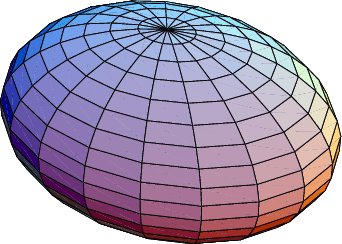
\includegraphics[scale=0.15]{ellipsoid}
\end{tabularx}

\begin{tabularx}{\linewidth}{@{}X@{}X@{}}
    \textbf{Hyperboloid of One Sheet}\newline
    $ \frac{x^2}{a^2}+\frac{y^2}{b^2}-\frac{z^2}{c^2} = 1 $\newline
    (Major Axis: z because it follows - )
    & 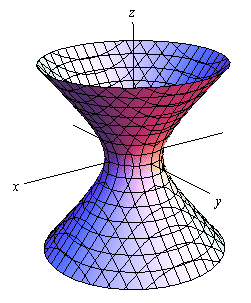
\includegraphics[scale=0.15]{hyperboloid1}
\end{tabularx}

\begin{tabularx}{\linewidth}{@{}X@{}X@{}}
    \textbf{Hyperboloid of Two Sheets}\newline
    $ \frac{z^2}{c^2}-\frac{x^2}{a^2}-\frac{y^2}{b^2} = 1 $\newline
    (Major Axis: Z because it is the one not subtracted)
    & 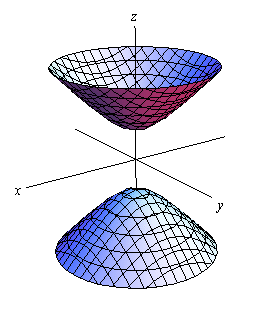
\includegraphics[scale=0.15]{hyperboloid2}
\end{tabularx}

\begin{tabularx}{\linewidth}{@{}X@{}X@{}}
    \textbf{Elliptic Paraboloid}\newline
    $ z=\frac{x^2}{a^2}+\frac{y^2}{b^2} $\newline
    (Major Axis: z because it is the variable NOT squared)
    & 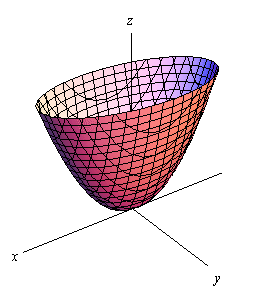
\includegraphics[scale=0.15]{elliptic_paraboloid}
\end{tabularx}

\begin{tabularx}{\linewidth}{@{}X@{}X@{}}
    \textbf{Hyperbolic Paraboloid}\newline
    (MA: Z axis because it is not squared)\newline
    $ z=\frac{y^2}{b^2}-\frac{x^2}{a^2} $
    & 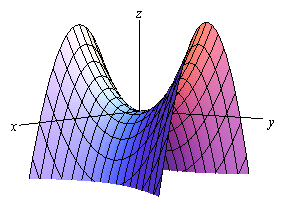
\includegraphics[scale=0.15]{hyperbolic_paraboloid}
\end{tabularx}

\begin{tabularx}{\linewidth}{@{}X@{}X@{}}
    \textbf{Elliptic Cone}\newline
    (Major Axis: Z axis because it's the only one being subtracted)\newline
    $ \frac{x^2}{a^2}+\frac{y^2}{b^2}-\frac{z^2}{c^2} = 0 $
    & 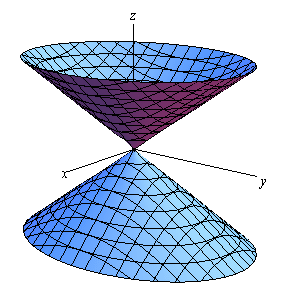
\includegraphics[scale=0.15]{elliptic_cone}
\end{tabularx}

\textbf{Cylinder}\newline
1 of the variables is missing\newline
OR 
$ (x-a)^2+(y-b^2) = c $\newline
(Major Axis is missing variable)

\subsection { Coord Systems }
Remember the Jacobian!!\newline
\textbf{Cylindrical to Rectangular}\newline
$ x=r\cos(\theta) $; $ y=r\sin(\theta) $; $ z=z $\newline
\textbf{Rectangular to Cylindrical}\newline
$ r=\sqrt{x^2+y^2} $; $ \tan(\theta) = \frac{y}{x} $; $ z=z $\newline
\textbf{Spherical to Rectangular}\newline
$ x=\rho\sin(\phi)\cos(\theta) $; $ y=\rho\sin(\phi)\sin(\theta) $; $ z=\rho\cos(\phi) $\newline
\textbf{Rectangular to Spherical}\newline
$ \rho=\sqrt{x^2+y^2+z^2} $; $ \tan(\theta) = \frac{y}{x} $; $ \cos(\phi) = \frac{z}{\sqrt{x^2+y^2+z^2}} $\newline
\textbf{Spherical to Cylindrical}\newline
$ r=\rho\sin(\phi) $; $ \theta=\theta $; $ z=\rho\cos(\phi) $\newline
\textbf{Cylindrical to Spherical}\newline
$ \rho=\sqrt{r^2+z^2} $; $ \theta=\theta $; $ \cos(\phi) = \frac{z}{\sqrt{r^2+z^2}} $

\columnbreak

\section{Derivatives}
$D_x e^x=e^x$\newline
$D_x \sin(x)=\cos(x)$\newline
$D_x \cos(x)=-\sin(x)$\newline
$D_x \tan(x)=\sec^2(x)$\newline
$D_x \cot(x)=-\csc^2(x)$\newline
$D_x \sec(x)=\sec(x)\tan(x)$\newline
$D_x \csc(x)=-\csc(x)\cot(x)$\newline
$D_x \sin^{-1}=\frac{1}{\sqrt{1-x^2}}, x \in [-1,1]$\newline
$D_x \cos^{-1}=\frac{-1}{\sqrt{1-x^2}}, x \in [-1,1]$\newline
$D_x \tan^{-1}=\frac{1}{1+x^2}, \frac{-\pi}{2}\le x \le \frac{\pi}{2}$\newline
$D_x \sec^{-1}=\frac{1}{\mid x \mid \sqrt{x^2-1}}, |x| > 1$\newline
% $D_x \sinh(x)=\cosh(x)$\newline
% $D_x \cosh(x)=\sinh(x)$\newline
% $D_x \tanh(x)=sech^2(x)$\newline
% $D_x \coth(x)=-csch^2(x)$\newline
% $D_x sech(x)=-sech(x)\tanh(x)$\newline
% $D_x csch(x)=-csch(x)\coth(x)$\newline
% $D_x \sinh^{-1}=\frac{1}{\sqrt{x^2+1}}$\newline
% $D_x \cosh^{-1}=\frac{-1}{\sqrt{x^2-1}}, x > 1$\newline
% $D_x \tanh^{-1}=\frac{1}{1-x^2} -1 < x < 1$\newline
% $D_x sech^{-1}=\frac{1}{x \sqrt{1-x^2}}, 0 < x < 1$
$ D_x \ln(x) = \frac{1}{x} $\newline

\textbf{Product rule}\newline
$ \frac{d}{dt} a \cdot b = a'b + ab' $

\section{Integrals}
$\int \frac{1}{x}dx = \ln|x|+c$\newline
$\int e^x dx = e^x+c $\newline
$\int a^x dx = \frac{1}{\ln a} a^x+c $\newline
$\int e^{ax} dx = \frac{1}{a} e^{ax}+c $\newline
$\int \frac{1}{\sqrt{1-x^2}} dx = \sin^{-1}(x)+c $\newline
$\int \frac{1}{1+x^2} dx = \tan^{-1}(x)+c $\newline
$\int \frac{1}{x\sqrt{x^2-1}} dx = \sec^{-1}(x)+c $\newline
% $\int \sinh(x) dx = \cosh(x)+c $\newline
% $\int \cosh(x) dx = \sinh(x)+c $\newline
% $\int \tanh(x) dx = \ln|\cosh(x)|+c $\newline
% $\int \tanh(x)sech(x) dx = -sech(x)+c $\newline
% $\int sech^2(x) dx = \tanh(x)+c $\newline
% $\int csch(x)\coth(x) dx = -csch(x)+c $\newline
$\int \tan(x) dx = -\ln|\cos(x) |+c $\newline
$\int \cot(x) dx = \ln|\sin(x)|+c $\newline
$\int \cos(x) dx = \sin(x)+c $\newline
$\int \sin(x) dx = -\cos(x)+c $\newline
$\int \frac{1}{\sqrt{a^2-u^2}} dx = \sin^{-1}(\frac{u}{a})+c $\newline
$\int \frac{1}{a^2+u^2} dx = \frac{1}{a}\tan^{-1}\frac{u}{a}+c $\newline
$ \int ln(x) dx = (xln(x))-x+c $\newline

\textbf{U-Substitution}\newline
Let $ u=f(x) $ (can be more than one variable).\newline
Determine: $ du = \frac{f(x)}{dx}dx $ and solve for dx.\newline
Then, if a definite integral, substitute the bounds for $ u=f(x) $ at each bounds\newline
Solve the integral using u.\newline

\textbf{Integration by Parts}\newline
$ \int u dv = uv-\int v du $

\section{Fns and Identities}
$\sin(\cos^{-1}(x)) = \sqrt{1-x^2}$\newline
$\cos(\sin^{-1}(x)) = \sqrt{1-x^2} $\newline
$\sec(\tan^{-1}(x)) = \sqrt{1+x^2} $\newline
$\tan(\sec^{-1}(x)) \newline = (\sqrt{x^2-1} \: $if$ \: x \ge 1)\newline =(-\sqrt{x^2-1} \: if \: x \le -1)$
% $\sinh^{-1}(x) = \ln{x+\sqrt{x^2+1}} $\newline
% $\sinh^{-1}(x) = \ln{x+\sqrt{x^2-1}}, \: x \ge -1 $\newline
% $\tanh^{-1}(x) = \frac{1}{2}\ln{x+\frac{1+x}{1-x}}, \: 1 < x < -1 $\newline
% $sech^{-1}(x) = \ln[{\frac{1+\sqrt{1-x^2}}{x}}], \: 0 < x \le -1 $\newline
% $\sinh(x) = \frac{e^{x}-e^{-x}}{2} $\newline
% $\cosh(x) = \frac{e^{x}+e^{-x}}{2} $

\section{Trig Identities}
$ \sin^2(x)+\cos^2(x) = 1 $\newline
$ 1+\tan^2(x) = \sec^2(x) $\newline
$ 1+\cot^2(x) = \csc^2(x) $\newline
$ \sin(x\pm y) = \sin(x)\cos(y)\pm\cos(x)\sin(y) $\newline
$ \cos(x\pm y) = \cos(x)\cos(y)\pm\sin(x)\sin(y) $\newline
$ \tan(x\pm y) = \frac{\tan(x)\pm\tan(y)}{1 \mp \tan(x)\tan(y)} $\newline
$ \sin(2x) = 2\sin(x)\cos(x) $\newline
$ \cos(2x) = \cos^{2}(x) - \sin^{2}(x) $\newline
% $ \cosh(n^{2}x)-\sinh^{2}x = 1 $\newline
$ 1+\tan^2(x) = \sec^2(x) $\newline
$ 1+\cot^2(x) = \csc^2(x) $\newline
$ \sin^2(x) = \frac{1-\cos(2x)}{2} $\newline
$ \cos^2(x) = \frac{1+\cos(2x)}{2} $\newline
$ \tan^2(x) = \frac{1-\cos(2x)}{1+\cos(2x)} $\newline
$ \sin(-x) = -\sin(x) $\newline
$ \cos(-x) = \cos(x) $\newline
$ \tan(-x) = -\tan(x) $

\end{multicols*}
\end{document}
